\subsection{Пилотное измерение энергии всей платы через USB}
\label{sec:energy-pilot}
Методические ориентиры для энергии встроенного ML задают MLPerf Tiny~\cite{Banbury2021MLPerfTiny} и ULPMark-CoreMark~\cite{EEMBCULPMarkCM}. MLPerf Tiny использует повторяемый вывод в течение не менее 10~с, энергию того же временного интервала и медиану пяти повторов. Здесь две записи на реализацию и плату, мощность центрального окна и полная длительность партии MCU; это другой исследовательский протокол. Ссылки дают контекст определения границы измерения и не означают соблюдения стандартного бенчмарка или сертификации ULPMark.

Для оценки затрат энергии проведена отдельная серия 15 сентября 2026 года: пять зафиксированных реализаций, по две записи на каждом из тех же экземпляров Mega 2560 и ESP32-C3, всего двадцать записей. USB-тестер FNIRSI FNB58, серийный номер 104332, включён последовательно в цепь питания платы (рис.~\ref{fig:energy-setup}). Мощность относится ко всей нагрузке после точки измерения, включая потери соединительного кабеля. Сохранённая USB-идентичность связывает серию ESP32-C3 с ранее использованной платой. Потребление платы в состоянии ожидания не вычитается. Поэтому результат не является энергией одного процессорного ядра или только арифметических операций модели.

\begin{figure}[!htbp]
\centering
\begin{minipage}[t]{0.46\textwidth}
\centering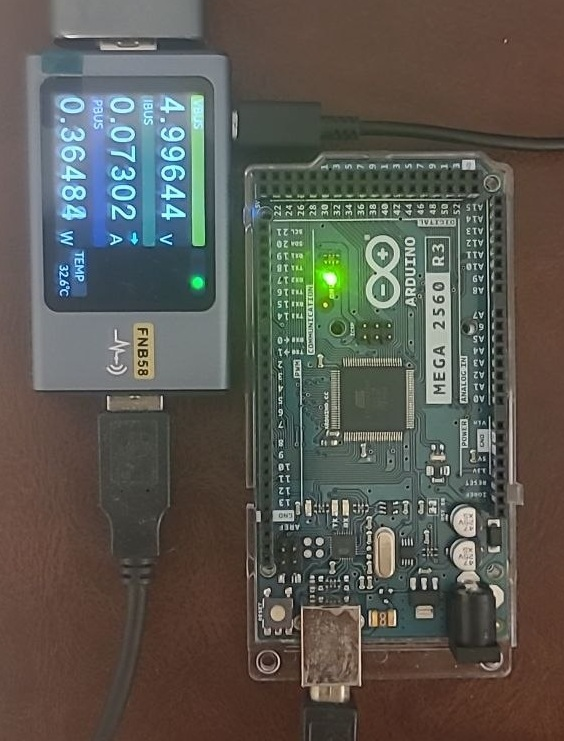
\includegraphics[height=5cm]{figures/Mega_measurement.jpg}\\[2pt]
\small (a) Arduino Mega 2560
\end{minipage}\hfill
\begin{minipage}[t]{0.46\textwidth}
\centering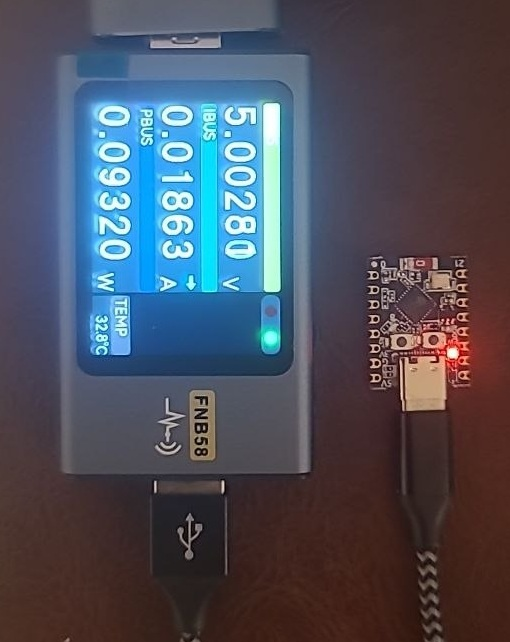
\includegraphics[height=5cm]{figures/C3_measurement.jpg}\\[2pt]
\small (b) ESP32-C3
\end{minipage}
\caption{Подключение плат к USB-тестеру FNB58. Фотографии иллюстрируют измерительную установку; показания на экранах являются отдельными снимками и не представляют средние активных вычислительных интервалов. Исполненная прошивка, модель и идентификатор платы устанавливаются по журналам и двоичным файлам, а не по фотографиям.}
\label{fig:energy-setup}
\end{figure}

Активная партия циклически повторяет двадцать общих исходных потоков в собственных зафиксированных представлениях каждой модели. Признаки заранее подготовлены в RAM; миллионы вызовов не означают миллионы различных наблюдений. После прогрева и калибровки число вызовов $N$ выбирается для партии продолжительностью около 120~с. Время $T_{\rm MCU}$ определяется по отметкам микроконтроллера вокруг всей партии, без таймера на каждом вызове. Оно включает цикл, индексацию входов, накопление контрольной суммы и обслуживание прерываний. Подготовка признаков, последовательный вывод и световые маркеры выполняются вне активной партии. Следовательно, $T_{\rm MCU}/N$ характеризует средние затраты вызова внутри партии; его нельзя подменять задержкой отдельного вызова из исходного протокола с 500 потоками.

В серии C3 модели выполняются в порядке: коэффициенты, LUT, MLP, многослойная KAN, DT5. Каждая пара записей получена после одной загрузки прошивки, с повторными подготовкой и калибровкой, но без холодного перезапуска платы между записями. Частота CPU составляет 160~МГц; Wi-Fi и Bluetooth не инициализированы, прерывания разрешены, явного \texttt{yield} в активном цикле нет. Используется 64-битный \texttt{esp\_timer\_get\_time}. Журналы всех десяти опытов C3 показывают отсутствие проверяемых подписок задач loop и idle на сторожевой таймер до измерения и ноль временно снятых подписок: предусмотренный прошивкой условный механизм снятия здесь не потребовался. Проверка фактических ELF/BIN подтверждает наличие настоящего вызова модели внутри счётного цикла во всех пяти вариантах. Константы моделей совпадают с зафиксированными заголовками и размещены во Flash; входы находятся в RAM. Двадцать подготовленных предсказаний отдельно сверяются со скомпилированным эталоном; для активной партии проверяется ожидаемая сумма бинарных ответов. Такая контрольная сумма не является отдельной проверкой каждого из миллионов решений.

Точная индексация LUT для этих двадцати входов обращается к 208 из 10,250 числовых ячеек (2.03\%, 416 байт табличного payload); для 500 потоков --- к 1,425 ячейкам (13.90\%, 2,850 байт). Это количество адресуемых ячеек, а не измеренный cache footprint: строки кеша, ассоциативность и промахи отдельно не установлены. Многократное повторение малого набора благоприятно для прогрева, поэтому пилотный вывод ограничен именно двадцатью входами.

Перед активной партией и после неё записывается световой код из трёх импульсов длительностью 2, 4 и 2~с. Для каждого CFN-файла двенадцать центров фронтов двух кодов задают отдельное аффинное соответствие времени прибора и MCU. В C3 небольшой сигнал светодиода выделяется в низкотоковых областях по обе стороны вычислительного интервала; большой подъём тока при вычислении не используется вместо световых фронтов. Средняя мощность определяется в заранее выбранных центральных 60~с активной партии по времени MCU. Если $[a,b]$ --- соответствующий интервал на временной оси CFN, то
\begin{equation}
\overline P=\frac{1}{b-a}\int_a^b V(t)I(t)\,dt,
\qquad
\widehat E_{\rm call}=\overline P\frac{T_{\rm MCU}}{N}.
\label{eq:energy-pilot}
\end{equation}
Интеграл вычисляется методом трапеций по сохранённым произведениям $V I$ с линейной интерполяцией на границах окна. Поле PBUS сверяется с $V I$ как производный канал того же прибора; это внутренняя согласованность, а не независимая проверка точности. Версия прошивки измерителя и версия фактически установленного GUI не записаны. Зафиксированный CFN-декодер опирается на описание формата FNIRSI Toolbox v0.0.6; это ссылка на схему, а не подтверждение версии установленного ПО. Поле NRG даёт приблизительно четверть интеграла $V I$ и исключено из расчёта; эмпирическое умножение этого поля на четыре не применяется. Величина $\widehat E_{\rm call}$ является некалиброванной инженерной оценкой энергии всей измеряемой итерации (ядро, цикл, индексация, контрольная сумма, прерывания и фоновое потребление) по стационарной мощности, а не точным интегралом всей активной партии или непосредственно разрешённой прибором энергией микросекундного вызова.

\begin{table}[!htbp]
\centering\footnotesize\setlength{\tabcolsep}{4pt}
\caption{Отдельная пилотная серия: среднее время внутри партии, USB-мощность всей платы и инженерная оценка энергии всей измеряемой итерации. Каждая строка и плата обобщают две записи с одинаковым весом. Энергия сначала вычисляется для каждой записи, затем усредняется. Числа округлены; полная точность сохранена в CSV. Исторические измерения времени в эту таблицу не включены.}
\label{tab:energy-pilot}
\begin{tabular}{lrrrrrr}
\toprule
& \multicolumn{3}{c}{Mega 2560, 16~МГц} & \multicolumn{3}{c}{ESP32-C3, 160~МГц}\\
\cmidrule(lr){2-4}\cmidrule(lr){5-7}
Реализация & мкс/вызов & мВт & мкДж/вызов & мкс/вызов & мВт & мкДж/вызов\\
\midrule
KAN, коэфф. & 1395 & 353 & 493 & 5.21 & 168 & 0.875\\
KAN, LUT & 225 & 354 & 79.6 & 3.33 & 166 & 0.552\\
Многосл. KAN & 12224 & 355 & 4342 & 54.2 & 174 & 9.42\\
MLP16 & 1341 & 356 & 477 & 19.8 & 170 & 3.37\\
DT5 & 15.7 & 358 & 5.63 & 0.739 & 169 & 0.125\\
\bottomrule
\end{tabular}
\end{table}

\begin{figure}[!htbp]
\centering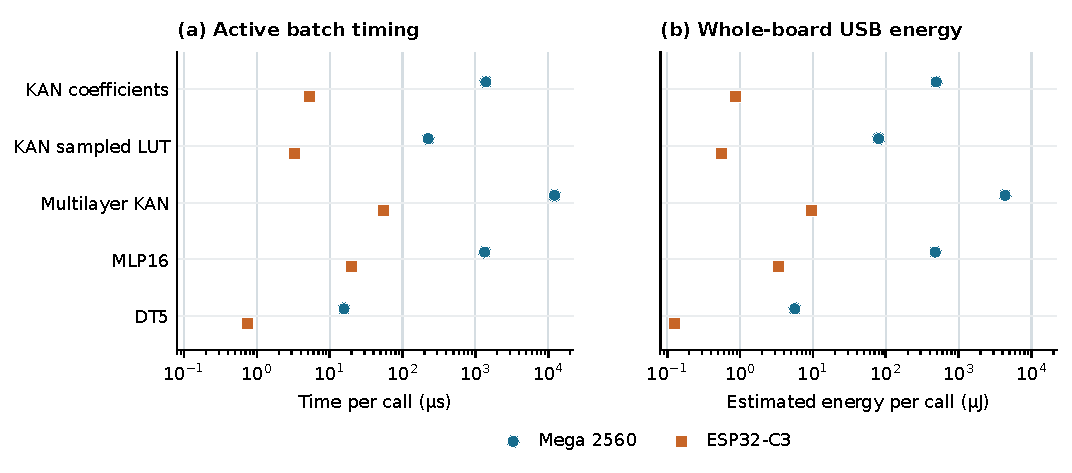
\includegraphics[width=\textwidth]{figures/energy_pilot_comparison.pdf}
\caption{Пилотная серия на двух платах: среднее время вызова внутри активной партии и оценка USB-энергии всей платы на вызов. Использованы логарифмические шкалы; отметки средних обобщают по две записи. Различия плат включают частоту CPU, архитектуру, компилятор, память и среду исполнения; график не выделяет эффект одной только системы команд.}
\label{fig:energy-pilot}
\end{figure}

Результаты приведены в табл.~\ref{tab:energy-pilot} и на рис.~\ref{fig:energy-pilot}. На Mega переход от коэффициентов к LUT сокращает время внутри партии на 83.88\% и энергию на вызов на 83.83\%; отношение коэффициентного значения к табличному составляет соответственно 6.205 и 6.186. На C3 сокращения равны 36.19\% и 36.94\%, а отношения --- 1.567 и 1.586. Мощность этих двух режимов близка в пределах каждой платы, поэтому основной наблюдаемый выигрыш энергии связан с более коротким вычислением. DT5 имеет наименьшие время и энергию в данной серии, но она не измеряет качество классификации и не устанавливает лучшее соотношение качества и ресурсов для произвольной задачи.

Относительное расхождение двух оценок энергии каждой модели C3, вычисленное как $(E_2/E_1-1)100\%$, по модулю меньше 0.09\%; для моделей Mega оно меньше 0.32\%. Более длинное внутреннее окно отличается от центральных 60~с менее чем на 0.048\% по всем двадцати записям. На C3 сдвиг центрального окна на $\pm2$~с изменяет среднюю мощность не более чем на 0.0151\%. Это описательные проверки повторяемости и устойчивости окна, а не абсолютная точность прибора. Прибор и часы MCU независимо не калиброваны; постоянная задержка измерительного тракта по этой привязке не определяется. Наблюдаемый фронт растянут примерно на одну секунду, поэтому сетка сохранения 0.1~с не устанавливает полосу измерения 10~Гц. Коррелированные отсчёты CFN не рассматриваются как независимые повторы для доверительных интервалов. Фиксированный порядок, одна плата каждого типа и два получения записи ограничивают обобщение результатов.

\begin{table}[!htbp]
\centering\footnotesize\setlength{\tabcolsep}{5pt}
\caption{Память фактически измеренных пилотных прошивок, байт. Показатель занятой Flash по PlatformIO, статические данные и длина BIN приложения являются различными величинами. Представления моделей сохраняют размеры из табл.~\ref{tab:memory}.}
\label{tab:energy-memory}
\begin{tabular}{lrrrrr}
\toprule
& \multicolumn{2}{c}{Mega 2560} & \multicolumn{3}{c}{ESP32-C3}\\
\cmidrule(lr){2-3}\cmidrule(lr){4-6}
Реализация & Flash & Данные и BSS & Flash по PIO & Данные и BSS & BIN\\
\midrule
KAN, коэффициенты & 22300 & 841 & 267790 & 15888 & 283856\\
KAN, LUT & 42060 & 841 & 287962 & 15888 & 300016\\
Многослойная KAN & 28266 & 841 & 273118 & 15904 & 285248\\
MLP16 & 22310 & 841 & 268144 & 15888 & 283728\\
DT5 & 23232 & 917 & 269486 & 15968 & 283520\\
\bottomrule
\end{tabular}
\smallnote{Во всех пяти C3-прошивках дополнительно 47\,906 байт кода в instruction RAM и 222 байта выравнивания. Перекрывающее адресное представление \texttt{.dram0.dummy} повторно не суммируется. Эти показатели не измеряют пики стека и кучи.}
\end{table}

Цена перехода к LUT на C3 --- рост занятой Flash пилотного приложения с 267\,790 до 287\,962 байт при увеличении представления модели с 254 до 20\,554 байт (табл.~\ref{tab:energy-memory}). Представление MLP занимает 760 байт, из которых 756 сохраняются отдельными объектами ELF; четырёхбайтовое смещение встроено компилятором в инструкции, и его значение проверено. Статические размеры и успешное исполнение не заменяют измерения пикового использования SRAM. Далее сохранён отдельный учёт памяти исторических приложений.
